\documentclass[a4paper, 12pt]{article}
\usepackage{graphicx}
\usepackage[a4paper,top=3cm,bottom=2cm,left=2cm,right=2cm,marginparwidth=2.5cm]{geometry}
\usepackage[utf8]{inputenc}
\usepackage[colorlinks=true, linkcolor=blue]{hyperref}


\title{OpenMP}
\author{Alessandro Castelli}
\date{\today}

\begin{document}

\maketitle

\section{Cos'è}
\textbf{OpenMP} è un'interfaccia di programmazione di applicazioni che supporta la programazzione multi processore.
È nativamente supporta da: \textbf{C, C++, Fortan}.
Per capire come funziona guarda la Figura \ref{fig:ForkJoin}, in cui è visibile come agisca attraverso un metodo \texttt{Fork-Join}.

\begin{figure}[h]
    \centering
    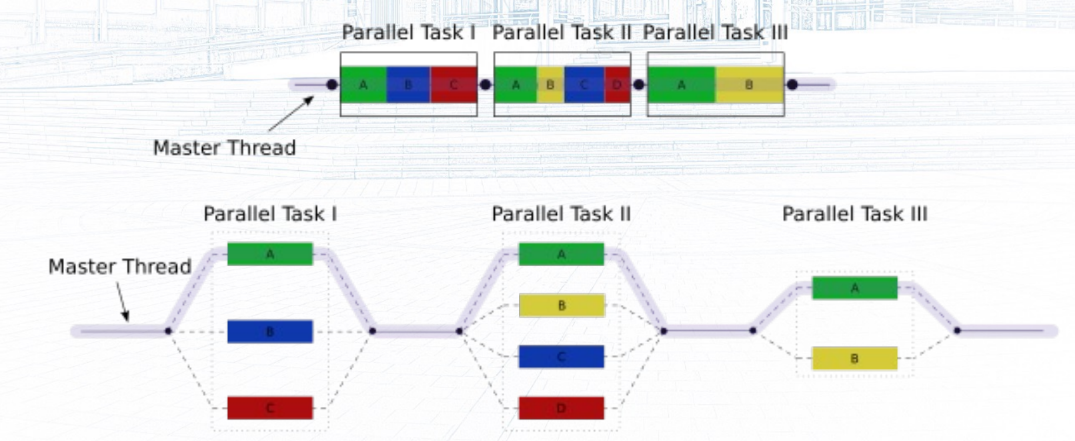
\includegraphics[width=0.5\textwidth]{ForkJoin.png}
    \caption{Fork-Join}
    \label{fig:ForkJoin}
\end{figure} 

\section{OpenMP memory }
\begin{itemize}
    \item \textbf{Shared memory model}: thread comunicano tramite accesso a variabili condivise.
    \item \textbf{La condivisione è definita sinitatticamente}
    \item \textbf{Sono possibili le \texttt{Race Conditions}}
\end{itemize}
\end{document}
